\documentclass[12pt,a4paper]{article}
\usepackage{color,graphics,amsmath,rotating}
\textheight=24cm
\textwidth=16cm
\oddsidemargin 0cm
\topmargin 0cm
\headsep 0cm
\pagestyle{plain}
\bibliographystyle{unsrt}

\usepackage{color}

\begin{document}

\def\micro{{\tt micrOMEGAs}}
\def\ra{\rightarrow}
\def\calchep{{\tt CalcHEP}}

\def\suspect{{\tt SuSpect}}
\def\mbmb{m_b(m_b)}
\def\mt{m_t}
\def\dMb{\Delta m_b}
\def\dMq{\Delta m_q}
\def\delrho{\Delta\rho}
\def\bsgamma{b\to s\gamma}
\def\bsmu{B_s\to \mu^+\mu^-}
\def\gmuon{(g-2)_\mu}
\def\noi{\noindent}


\begin{flushright}
   \vspace*{-18mm}
   Date: \today
\end{flushright}
\vspace*{2mm}




\begin{center}


{\Large\bf The  micrOMEGAs user's manual, version 2.4} \\[8mm]

{\large   G.~B\'elanger$^1$, F.~Boudjema$^1$, A.~Pukhov$^2$,  A. Semenov$^3$.}\\[4mm]

{\it 1) LAPTH, Univ. de Savoie, CNRS, B.P.110,  F-74941 Annecy-le-Vieux, France\\
     2) Skobeltsyn Inst. of Nuclear Physics, Moscow State Univ., Moscow 119992, Russia\\
     3) Joint Institute for Nuclear Research (JINR) 141980, Dubna,  Russia\\}
\end{center}

\begin{abstract}
We give an up-to-date description of micrOMEGAs functions. Only the routines which are available for
the users are described.  Examples on how to use these functions
can be found in the sample main programs distributed with the code. 
\end{abstract}




\section{Introduction}
\micro~ is a code 
 to calculate the properties of cold dark matter  in a generic model of particle physics.  
 First developed to compute the relic density of dark matter, 
 the code also computes the rates for dark matter direct and  indirect detection. 
 It is assumed that a discrete symmetry like R-parity ensures the stability of the lightest 
 odd particle (LOP). 
All annihilation and coannihilation channels are included in the computation of the relic density. 
This manual gives an up-to-date description of all \micro~ functions.  
The method used to compute the dark matter properties are described 
in references 
~\cite{Belanger:2001fz,Belanger:2004yn,Belanger:2006is,Belanger:2008sj}.
These references also contain  a more complete description of the code. In the following
the cold dark matter candidate also called LOP or weakly-interactive massive particle (WIMP)
will be denoted by $\chi$. 

\micro~ contains both C and Fortran routines. Below we describe only the
C-version of the routines,  in general we use the same  names
 and the same types of argument for both  C and Fortran funtions. 
We always use \verb|double(real*8)| variables for float point numbers and 
\verb|int(INTEGER)| for integers. In this manual we use {\it FD} for a file descriptor 
variables, the file descriptors  are  \verb|FILE*| in C and {\tt channel number} in Fortran. 
The symbol \verb|&| before the names of variables in C-functions stands for 
the address of the variable. It is used for  {\it output
parameters}. In Fortran calls there is no need for \verb|&|
since  all parameters are passed via addresses. In C programs one  can substitute {\tt
NULL} for output parameters which the user chooses to ignore. In Fortran  one
can substitute {\tt cNull, iNull, r8Null} for unneeded
parameters of  {\it character}, {\it integer}  and {\it real*8}  type respectively.  

A few C-functions use pointer variables that specify an {\it address} in 
the computer memory. Because pointers do not exist in  Fortran one uses any
other type of variable whose length os sufficient to store a computer address 
(4 or 8 bytes), for example an {\it INTEGER*4} array with length 2 or 
a {REAL*8} variable. 

The complete format  for all functions can be found in
\verb|sources/micromegas.h| (for C) or
\verb|sources/micromegas_f.h| (for Fortran). Examples on how to use these functions are provided   
in the MSSM/main.c[F] file. 
 
 
 \micro~ assumes that all particles that are odd under the discrete symmetry have
 a name starting with '\verb|~|', for example \verb|~o1| for the lightest  neutralino.
\newpage

\section{ Global Parameters}
%\label{global_parameters}
The list of global parameters and their default values are given in Table
\ref{paramTab}. 
The use of global parameters is
a new feature of version 2.4 of \micro.

\begin{table}[h]
 \caption{Global parameters of micrOMEGAs}
 \label{paramTab}
\begin{center}
\begin{tabular}{|l|l|l|l|l|}
\hline
  Name      &default value & units &  comments \\  \hline
  Mcdm      &              &  GeV  & Mass of Dark Matter particle           \\ 
ScalarFFPd  &  0.03302     &       & \\
ScalarFFPu  &  0.02348     &       & Scalar form factor for quark in proton\\
ScalarFFPs  &  0.2594      &       & \\
pVectorFFPd &  -0.427      &       & Axial-vector form factor for quark in proton\\
pVectorFFPu &   0.842      &       & \\
pVectorFFPs &  -0.085      &       & \\
SigmaFFPd   &  -0.23       &       & Tensor form factor of d-quark in proton\\
SigmaFFPu   &   0.84       &       & \\
SigmaFFPs   &   -0.046     &       & \\
ScalarFFNd  &  0.04241     &       & Scalar form factor of d-quark in neutron\\
ScalarFFNu  &  0.01823     &       & \\
ScalarFFNs  &  0.2594      &       & \\
pVectorFFNd &  0.842       &       & \\
pVectorFFNu &  -0.427      &       & Axial-vector form factor for quark in proton\\
pVectorFFNs &  -0.085      &       & \\
SigmaFFNd   &  0.84        &       & \\
SigmaFFNu   &  -0.23       &       & \\
SigmaFFNs   &  -0.046      &       & \\
Fermi\_a    &  0.52        &  fm   & nuclei  surface thickness \\
Fermi\_b    &  -0.6        &  fm   &  parameters to set the nuclei radius with  \\    
Fermi\_c    &  1.23        &  fm   &  $R_A=c A^{1/3} +b$ \\ 
Rsun        & 8.5          & kpc   & Distance from Sun to center of Galaxy\\
Rdisk       & 20           & kpc   & Radius of galactic diffusion disk \\
rhoDM       &  0.3         & $GeV/cm^3$ & Dark Matter density at Rsun\\
Vearth      &  225.2   & km/s     & Galaxy velocity of Earth     \\  
%K\_dif      & $3.10^{27}$ & $cm^2/s $ & The normalized diffusion coefficient \\
K\_dif      & 0.0112     & $kpc^2/Myr$ & The normalized diffusion coefficient\\
L\_dif      & 4           & kpc       & Vertical size of Galaxy diffisive halo \\
Delta\_dif   & 0.7        &           &Slope of diffision coefficient\\ 
Tau\_dif    & $10^{16}$   &   s       &Electron energy loss time\\
Vc\_dif     & 0           &  km/s     &  Convective Galactic vind \\
\hline
\end{tabular}
\end{center}
\end{table}



\section{Setting of parameters, spectrum calculation, parameter display.}
\label{setting_parameters}
The independent parameters that characterize a given model are listed in 
the file \\
\noindent
\verb|work/models/vars1.mdl|. Three functions can be used to set the
value of these parameters:\\

\noindent
$\bullet$ \verb|assignVal(name,val)|\\
$\bullet$ \verb|assignValW(name,val)|\\
assigns value {\it val} to parameter {\it name}. The function  \verb|assignVal| returns a non-zero
value  if it
cannot recognize  a parameter name while \verb|assignValW| writes an error message.  \\
$\bullet$ \verb|readVar(fileName)|\\
reads parameters from a file. The file  should contain two columns with the 
 following  format 
\begin{verbatim}
    name    value
\end{verbatim}
\verb|readVar| returns zero when
the file has been read successfully, a negative value when the
file cannot be opened for reading and  a positive  value 
corresponding to the line where a wrong file record was found.

Note that in  Fortran, numerical constants should be specified as  Real*8, for example
\begin{verbatim}     
        call assignValW('SW', 0.473D0) 
\end{verbatim}
A common mistake is to use Real*4.  


The constrained parameters of the model are stored in \verb|work/models/func1.mdl|. Some of
these parameters are treated as {\it public} parameters. The {\it public} parameters include 
by default all particle masses 
and all parameters  whose calculation requires external functions (except simple
mathematical functions like $\sin,\cos$ .. ). The parameters
listed above any {\it public} parameters in  \verb|work/models/func1.mdl|
are also treated as {\it public}. 
It is possible to enlarge the list of {\it public} parameters. For this
one has to add a  special record in \verb|work/models/func1.mdl|
\begin{verbatim}
%Local! |   
\end{verbatim}
Then all parameters listed above this record  become {\it public}. 
See example in
\begin{verbatim} 
         MSSM/work/models/func1.mdl 
\end{verbatim}

The calculation of the particle spectrum and of all  {\it public} model constraints 
is  done with:\\
\noindent
 $\bullet$ \verb|sortOddParticles(txt)|\\
which sorts the odd
particles with increasing  masses,  writes the name of the lightest odd particle 
in \verb|txt| and    assigns  the value of the mass  of
the lightest odd particle to the global parameter \verb|Mcdm|.
This routine returns a non zero error code for a
wrong set of parameters, for example parameters  for which some
constraint cannot be calculated.
The name of the corresponding constraint is
written in \verb|txt|. This routine has to be called after a reassignment of any input parameter.

\noindent 
$\bullet$ \verb|qNumbers(pName, &spin2,&charge3,&cdim)|\\
returns the quantum numbers for the particle \verb|pName|. Here \verb|spin2| is twice the spin of the particle; \verb|charge3| is 
three times the electric charge; \verb|cdim| is the  dimension of the representation
of $SU(3)_c$, it can be $1,3,-3$ or $8$. The parameters {\tt spin2, charge3, cdim} are 
variables of type {\tt int} and {\tt massPrt} should be {\tt double*}. The value returned 
is the {\tt PDG} code. If \verb|pName| does not correspond to any
particle of the model then \verb|qNumbers| returns zero.

\noindent
$\bullet$  \verb|nextOdd(n, &pMass)| \\
returns the name and mass of the $n^{th}$ odd particle assuming that particles are 
sorted according to increasing masses. For $n=0$ the output specifies the 
name and the mass of the CDM candidate. In the FORTRAN version this function 
is \verb|Subroutine nextOdd(n,pName,pMass)| 

\noindent
$\bullet$  \verb|pdg2name(nPDG)| \\
returns  the name of  the particle which PDG code is {\it nPDG}. If this particle does not exist in the model
the return value is NULL.  In the FORTRAN version this function
is \verb|Subroutine pdg2name(nPDG, pName)| and the character variable
\verb|pName| consists of white
spaces if the particle does not exist in the model. 

\noindent
$\bullet$  \verb|pMass(pName)| \\
returns  numerical value of the particle mass.

\noindent
$\bullet$ \verb|findVal(name,&val)|\\
 finds the  value of
 variable  {\it name} and assigns it to parameter {\it val}. It returns a non-zero
value  if it cannot recognize  a parameter name. \\
$\bullet$ \verb|findValW(name)| 
just returns the value of variable {\it name} and writes an error message
if it cannot recognize  a parameter name.
%\noindent
%$\bullet$ \verb| findVal(name,&val)|\\
%$\bullet$ \verb| findValW(name)|\\
The variables accessible by these commands are all free parameters and   the 
constrained parameters of the model (in file \verb|model/func1.mdl|)
treated as {\it public}. 

The following routines are used to display the value of independent and constrained 
{\it public}
parameters: 

%A check of model constrained parameters  can be done by\\ 

\noindent
$\bullet$ \verb|printVar(FD)|\\ 
prints the numerical values of all independent and {\it public} 
constrained parameters into \verb|FD|\\
$\bullet$ \verb|printMasses(FD, sort)|\\
 prints the masses of 'odd' particles
(those whose names  started with \verb|~|). If $sort\ne 0$
the masses are sorted so the mass of the CDM is given first.\\
$\bullet$ \verb|printHiggsMasses(FD, sort)|\\
prints the masses and widths of 'even' scalars.\\


\section{ Relic density calculation.}

$\bullet$ \verb|vSigma(T,Beps,fast)|\\
calculates the thermally averaged cross section for DM annihilation  times velocity  
at a  temperature T [GeV], see formula (2.6) in ~\cite{Belanger:2001fz}. The value for $\sigma v$ 
is expressed in [pb].  The parameter $Beps$ defines the criteria for including coannihilation
channels as for {\tt darkOmega} described below.
The $fast=1/0$ option switches between the {\it fast}/{\it accurate} calculation. 
The global array {\tt vSigmaTCh} contains the 
contribution of different channels to {\tt vSigma}. \verb|vSigmaTCh[i].weight| specifies the relative
weight of the $i^{th}$ channel \\
\verb|vSigmaTCh[i].prtc[j]|  {\it (j=0, 4)}  define particles names for the $i^{th}$
channel.\\
The last record in \verb|vSigmaTCh| array has zero weight and 
NULL particle names.  In the Fortran version, the function 
 \verb|vSigmaTCh(i,weight,particles)|serves the same purpose.  This function returns 0
if $i$  exceeds the number of annihilation  channels and 1 otherwise, $i\ge 1$. 
 {\it real*8 weight} gives the relative contribution of each
annihilation channel. {\it character*10 particles(4)} contains the names of
particles in the  annihilation process.\\ 
\noindent 
$\bullet$ \verb|darkOmega(&Xf,fast,Beps)|\\
calculates the dark matter relic density $\Omega h^2$. 
This routine  solves the differential evolution equation  using the Runge-Kutta method. 
$X_f=Mcdm/T_{f}$
characterizes the freeze-out temperature.   The value of $X_f$ is given for
information and is also used as an input for the routine that
gives the relative contribution of each channel to $\Omega h^2$,
see \verb|printChannels|  below. The  $fast=1$ flag forces the
fast calculation (for more details see
Ref.~\cite{Belanger:2004yn}). This is the recommended option and
gives an accuracy around $1\%$. The parameter {\tt Beps} defines the
criteria for including a given coannihilation channel in the computation of the
thermally averaged cross-section,~\cite{Belanger:2004yn}.   The
recommended value is $Beps=10^{-4} - 10^{-6}$, on the other hand
if $Beps=1$ only annihilation of the
lightest odd particle is computed.\\
\noindent
$\bullet$ \verb|darkOmegaFO(&Xf, fast,  Beps)|\\
calculates the  dark matter relic density $\Omega h^2$ using the freeze-out approximation.\\
\noindent
$\bullet$ \verb|printChannels(Xf,cut,Beps,prcnt,FD)|\\   
writes into \verb|FD| the  contributions  of different channels to $(\Omega
h^2)^{-1}$. Here \verb|Xf| is an input parameter which should
be first evaluated in \verb|darkOmega[FO]|. Only  the channels whose
relative contribution is larger than  \verb|cut| will be displayed. \verb|Beps|
plays the same role as the \verb|darkOmega[FO]| routine.
If $prcnt\ne 0$ the contributions are given in percent.
Note that  for this specific purpose  we use the
freeze-out approximation.\\
$\bullet$ \verb|oneChannel(Xf,Beps,p1,p2,p3,p4)|\\   
calculates the relative   contribution of the  channel $ p1,p2 \to p3,p4$
to $(\Omega h^2)^{-1}$  cohere  p1,...,p4 are particle names.  To make
summation over several channels one can substitute  \verb|"*"| instead 
of  a particle name.\\
\noindent
$\bullet$ \verb|omegaCh| is an array that contains the relative contribution and particle names for each
annihilation channel. In the Fortran version one uses instead
the function\\
\noindent\verb|omegaCh(i,weight,particles)|. These array and function
are similar to {\tt vSigmaTCh} described above. The array {\tt omegaCh} if filled after calling either
{\tt darkOmegaFO} or {\tt printChannels}. 





\section{Direct detection.}
\subsection{Amplitudes for elastic scattering}
\noindent
 $\bullet$ \verb|nucleonAmplitudes(qBOX,pAsi,pAsd,nAsi,nAsd)|\\
calculates the amplitudes for WIMP-nucleon elastic
scattering at zero momentum. \verb|pAsi(nAsi)| are spin
independent amplitudes for protons(neutrons) whereas
\verb|pAsd(nAsd)| are the corresponding spin dependent amplitudes.
Each of these four parameters is an array of 
dimension 2. The zeroth (first) element of these arrays gives the
$\chi$-nucleon amplitudes whereas the second element gives
$\overline{\chi}$-nucleon amplitudes. Amplitudes are normalized
such that the total cross section for either $\chi$ or $\overline
\chi$ cross sections is\footnote{All parameters in GeV.}
\begin{equation}
\sigma_{tot}=\frac{4M_{\chi}^2 M_N^2}{\pi(M_{\chi}+M_N)^2}(|A^{SI}|^2+3|A^{SD}|^2)
\label{eq:norm}
\end{equation}
If \verb|qBOX=NULL| (\verb|qBOX=NoLoop| in Fortran) tree level amplitudes are computed. 
In MSSM-type models with a spin 1/2 WIMP and scalar "squarks",   
\verb|qBOX=FeScLoop| uses  an improved tree-level calculation.  
\verb|nucleonAmplitudes| returns a value different from zero only
when there is an internal problem in calculation.


\verb|nucleonAmplitudes| depends implicitly on form factors which describe the 
quark contents in the nucleon. These form factors are global parameters (see
Table~\ref{paramTab} for
default values)
\begin{equation}
Type{\rm FFP}q \;\;\; Type{\rm FFN}q \nonumber
\end{equation} 
where $Type$ is either "Scalar", "pVector", or "Sigma",  FFP and FFN denote proton and neutron  and
$q$ specifies the quark, $d,u$  or $s$. Heavy quark coefficients are calculated automatically.

\noindent $\bullet$ \verb|getScalarFF(|$m_u/m_d,m_s/m_d,\sigma_{\pi
N},\sigma_0)$\\
computes the scalar coefficients for the quark contents in the
nucleon from the mass ratios $m_u/m_d,m_s/m_d$ as well as from
 $\sigma_{\pi N}$ and $\sigma_0$, the amplitudes for ${\pi N}$ scattering.
 $\sigma_{\pi N}$ and $\sigma_0$ should be specified in MeV.~\cite{Belanger:2008sj}
 
% \noindent
%$\bullet$ \verb|FeScLoop(sgn,mq,msq,mne)|\\
%computes the  loop K-factor for MSSM-like models with a
%spin 1/2 WIMP and a scalar "squark".  Here
%\verb|mq,msq,mne| refer to  quark, squark, and WIMP  masses,
%for details see ~\cite{Belanger:2008sj}.


\subsection{Scattering on nuclei}

$\bullet$ \verb|nucleusRecoil(f,A,Z,J,S00,S01,S11,qBOX,dNdE)|\\
This is the main routine of the  direct detection module. The
input parameters are:
\begin{itemize}
\item[$\diamond$]
\verb|f| -  the DM velocity distribution   normalized such that 
$$ \int_0^{\infty} v f(v) dv =1$$ 
The units  are $km/s$ for v and $s^2/km^2$ for  f(v).
\item[$\diamond$]
\verb|A| - atomic number of nucleus;
\item[$\diamond$]
\verb|Z| - number of protons in the nucleus, predefined values for a wide set of isotopes 
are called with $Z\_\{Name\}$;
\item[$\diamond$]
\verb|J| - nucleus spin,  predefined values for a wide set of isotopes
are called with\\
 $J\_\{Name\}\{atomic\_number\}$.
\item[$\diamond$]
\verb|S00, S01, S11| - nucleus form factors for
spin-dependent interactions. They  depend  of the momentum
transfer in $fm^{-1}$. The available form factors are
\begin{verbatim}
SxxF19   SxxNa23   SxxNa23A  SxxAl27   SxxSi29   SxxSi29A  
SxxK39   SxxGe73   SxxGe73A  SxxNb92   SxxTe125  SxxTe125A 
SxxI127  SxxI127A  SxxXe129  SxxXe129A 
SxxXe131 SxxXe131A SxxXe131B
\end{verbatim}
where $xx$ is either $00$, $11$ or $01$.  The last character 
is used to distinguish different implementations of
the form factor for the same isotope, see details in ~\cite{Belanger:2008sj}.
\item[$\diamond$]
\verb|qBOX| - a parameter needed by \verb|nucleonAmplitudes|, see the description above.
\end{itemize}
The form factors for the spin independent (SI) cross section are defined by a Fermi distribution
and depend on the global parameters \verb|Fermi_a|, \verb|Fermi_b|,
\verb|Fermi_c|. 

The returned value gives the number of events per day and per kilogram of 
detector material. The  result depends  implicitly on the  global  parameter \verb|rhoDM|, the
density of DM near the Earth.
The distribution over recoil energy is stored in the array 
$dNdE$ which by default has $Nstep=200$ elements.  
The value in the $i^{th}$ element corresponds to
$$
dNdE[i] = \frac{dN}{dE}|_{E=i*keV*step}
$$
in units of ${\rm (1/keV/kg/day)}$. By default $step$  is set to 1. 

For a complex WIMP, \verb|nucleusRecoil| averages over $\chi$ and
$\overline{\chi}$. For example for $^{73}Ge$, a call to this routine will be: 
\begin{verbatim}
nucleusRecoil(Maxwell,73,Z_Ge,J_Ge73,S00Ge73,S01Ge73,S11Ge73,FeScLoop,dNdE);
\end{verbatim}


\noindent
$\bullet$ \verb|setRecoilEnergyGrid(step,Nstep)| \\
changes the values of \verb|step| and \verb|Nstep| for the computation of \verb|dNdE|.


\noindent
$\bullet$ \verb|Maxwell(v)| \\
returns   
%$$ f(v)= \frac{c_{\rm{norm}}}{v}\left[
%exp\left(-\frac{(v-V_{earth})^2}{dv^2}\right) -
%exp\left(-\frac{min(v+V_{Earth},v_{max})^2}{dv^2}\right)\right] $$
$$f(\mbox{v})= \frac{c_{\rm{norm}}}{\mbox{v}}\int\limits_{|\vec{v}|<v_{max}} d^3\vec{v} \exp\left(
-\frac{(\vec{v}-V_{Earth})^2}{\Delta v^2}\right)\delta(\mbox{v} -|\vec{v}|)
$$
wich corresponds to the isothermal model. Default values
are  $\Delta v =220{\rm km/s}$,  $v_{max}=700{\rm km/s}$.$V_{Earth}$ is a global parameter
and $c_{norm}$ the normalization factor.  This function is an
argument of the \verb|nucleusRecoil| function described above.

\noindent
$\bullet$ \verb|SetfMaxwell(dv,vmax)|\\
sets parameters $\Delta v$ and $v_{max}$ for \verb|Maxwell|. 

\noindent
$\bullet$ \verb|nucleusRecoil0(f,A,Z,J,Sp,Sn,qBOX,dNdE)|\\
is similar to the  function \verb|nucleusRecoil| except that 
the spin dependent nuclei form factors are described by Gauss functions
whose values  at zero momentum transfer are defined by the coefficients \verb|Sp,Sn|~\cite{Belanger:2008sj}. 
Predefined values for the coefficients \verb|Sp,Sn| are included for the
nuclei listed in \verb|nucleusrecoil| as well as ${}^3He$, ${}^{133}Cs$. Their  names are 
\begin{eqnarray}
    &&Sp\_\{Nucleus\; Name\}\{Atomic \;Number\} \nonumber\\
    &&Sn\_\{Nucleus\; Name\}\{Atomic\; Number\} \nonumber
\end{eqnarray}
One can use this routine for nuclei whose form factors  are not known. 



\subsection{Auxiliary routines}
Two auxiliary routines are provided to work with the energy
spectrum computed with
\verb|nucleusRecoil| and  \verb|nucleusRecoil0|.\\
%
\noindent
$\bullet$ \verb|cutRecoilResult(dNdE,E1,E2)|\\
calculates the number of events in an energy interval defined by the
values \verb|E1,E2| in keV .

\noindent
$\bullet$ \verb|displayRecoilPlot(dNdE,title,E1,E2)|\\
plots the  generated energy distribution dNdE. Here \verb|title|
is a character string specifying the title of the plot and
\verb|E1,E2| are minimal and maximal values for the displayed
energy in keV.

\section{Indirect detection}

\subsection{ Interpolation and display of spectra}
Various spectra of particles relevant for indirect detection are stored in
arrays with {\bf NZ=250} elements. The $i^{th}$ element of an array corresponds to 
 $dN/dz_i$ where $z_i=log(E_i/Mcdm)$. Here $N$ stands for either 
 a number of particles or  a particle flux expressed in $(\rm{sec}\cdot{\rm cm}^2 {\rm
sr})^{-1}$.\footnote{
The value of $z_i$ can be obtained with the function 
$Zi(i)$. In the current version
$Zi(i)=log\left((10^{-7})^{(i/NZ)^{1.5}}\right)$. This function is in general not needed if one uses
the functions  described below.}

Table interpolation can be done by two functions\\ 
$\bullet$ \verb|zInterp(z,spectTab)| \\
or\\
$\bullet$  \verb|SpectdNdE(E,spectTab)|\\
interpolates the tabulated spectra  and returns the 
particle distribution \verb|dN/dE|  where \verb|E| is the energy  in GeV assumimg that 
$z=0$ corresponds to   \verb|E=Mcdm|.

To display the  spectra visualization one can use \\
$\bullet$ \verb|displaySpectrum(Spectrum,message,Emin,Emax,Units)|\\
displays the resulting spectrum, \verb|message| is a text string which gives a title to the  
plot. \verb|Emin| and \verb|Emax| define  energy cuts. If \verb|Units=0| the spectrum is written as a
function of $z=log_{10}(E/{\rm {Mcdm}})$ otherwise the spectrum is a function of the energy in GeV.



\subsection{Annihilation spectra}
$\bullet$ \verb|calcSpectrum(key,Sg,Se,Sp,Sne,Snm,Snl,&err)|\\
calculates  the spectra  of DM annihilation 
at rest and returns $\sigma v$ in $cm^3/s$ . The calculated spectra
for $\gamma$, $e^+$, $\bar{p}$, $\nu_e$, $\nu_{\mu}$, $\nu_{\tau}$ 
are stored in arrays of dimension \verb|NZ| as described above: \verb|Sg|, \verb|Se|, \verb|Sp|, 
\verb|Sg|, \verb|Sne|, \verb|Snm|, \verb|Snl|. 
 To remove the calculation of a given spectra, substitute  
\verb|NULL| for the corresponding argument. 
\verb|key| is a switch to include polarisation of W,Z bosons (\verb|key=1|) or
 photon radiation (\verb|key=2|).  Photon radiation is added to all subprocesses when computing the photon spectrum while
only the 3-body process $\chi\chi\rightarrow e^+e^-\gamma$ is included  for the positron spectrum. 
When \verb|key=4| the cross sections for each annihilation channel are written on the screen. More than one option
can be switched on simultaneously by adding the corresponding values for \verb|key|. 
For example both the W polarisation and photon radiation effects  are included if
\verb|key=3|.
A problem in the spectrum calculation will produce a non zero error code, $err\neq
0$. {\tt calcSpectrum} interpolates and sums spectra obtained
by Pythia. The spectra tables are provided only for Mcdm$>2$GeV. The results for a dark matter
mass below 2 GeV will therefore be wrong, for example an antiproton
spectrum  with  kinetically forbidden energies will be produced. A warning is issued for Mcdm$<2$GeV. \\  
$\bullet$ \verb|spectrInfo(Xmin,spectrTab,&Ntot,&Xtot)|\\
provides information on the spectra generated. Here \verb|Xmin| defines the minimum 
cut for the energy fraction x=E/Mcdm, \verb|Ntot| and \verb|Xtot| are calculated parameters 
which give on average the total number and the energy fraction of the final particles 
produced per collision. Note that the upper limit is Xtot=2.\\
$\bullet$ \verb|vSigmaCh| is an array that contains the relative contribution and particle names for each
annihilation channel. In the Fortran version one uses instead
the function\\
\noindent \verb|omegaCh(i,weight,particles)|. These array and function
are similar to {\tt vSigmaTCh} described above. The array {\tt vSigmaCh} if filled by 
{\tt calcSpectrum}.


\subsection{Distribution of Dark Matter  in Galaxy.}
To compute the signal from an indirect detection experiment one has 
to take into account the dark matter distribution in the Galaxy.
Usually the DM density is represented via a~{\it profile} function.
$$
   \rho(r)=\rho_\odot F_{halo}(r)     
$$
Dark Matter annihilation in the Galaxy depends on $<\rho^2>$ which
can be significantly larger than $<\rho>^2$ because of Dark Matter {\it
clumps}.  The effect of clumping can be described by another profile
\begin{equation}
<\rho^2>(r)=\rho^2_\odot F_{halo}^2(r)F_{clump}(r)
\end{equation}
The DM density at the Sun, $\rho\odot$,  is defined in micrOMEGAs by a
global variable \verb|rhoDM|.
\noindent
$\bullet$ \verb|setHaloProfiles(|$F_{halo},F_{clump}$\verb|)|\\
allows to change both the halo and the clump profile. Any sphericaly symmetric DM halo
profile can be defined.

\noindent
$\bullet$ \verb|noClumps(r)|\\
is  a non clumpy profile which is used by default. It returns $1$  for any argument. 

\noindent
$\bullet$ \verb|hProfileABG(r)|\\
is the default halo  density profile which is described by the function
\begin{equation}
\label{rho}
F_{halo}(r)=\left(\frac{ R_{sun}}{r}\right)^{\gamma}
\left(\frac{r_c^{\alpha}+ R_{sun}^{\alpha}}
{r_c^{\alpha}+r^{\alpha}}\right)^{\frac{\beta -\gamma}{\alpha}}
\end{equation}

\noindent
$\bullet$ \verb|setProfileABG(alpha,beta,gamma,a)|\\
resets the parameters  $\alpha=1,\beta=3,\gamma=1, rc=20[pc]$ of the default profile.
 
\noindent
$\bullet$ \verb|hProfileEinasto(r)|\\
is the Einasto halo density profile 
$$
F_{halo}(r)=exp\left[-\frac{2}{\alpha}\left((\frac{r}{R_{sun}})^{\alpha}-1\right)\right]
$$
  
\noindent
$\bullet$ \verb|setProfileEinasto(alpha)| \\
sets the parameter $\alpha$  for the  Einasto profile, the  default value is $\alpha=0.17$.



\subsection{Photon (neutrino) signal}
The photon  flux does not depend on the  diffusion model parameters but on the angle
$\phi$ between the line of sight and the center of the galaxy as well as on the annihilation spectrum
into photons

\noindent
$\bullet$ \verb|gammaFluxTab(fi,dfi,sigmav,Sg,Sobs)|\\
multiplies the annihilation photon spectrum  with the integral over the line of sight
and over the opening angle to give the photon flux. 
%\verb|fi| is the angle between the line of sight 
%and over angle of sight.
\verb|fi| is the angle between the line of sight and the center of the
galaxy,   \verb|dfi| is half the cone angle which characterizes the detector resolution
(the solid angle is  $2\pi (1-cos(dfi)$) ,  
 \verb|sigmav| is the annihilation cross section, \verb|Sg| is the DM annihilation spectra.
\verb|Sobs| is the spectra observed.


The function \verb|gammaFluxTab| can be used  for the neutrino spectra as well.

\noindent
$\bullet$ \verb|gammaFlux(fi,dfi,vcs)|\\
is the same function as \verb|gammaFluxTab| above  but corresponds to  
a discrete photon spectrum. \verb|vcs| is the annihilation cross section, for instance in the {\t MSSM} it is 
calculated with the \verb|loopGamma| function. The function
returns the number of photons per $cm^2$ of detector surface
 per second. Note that for $\chi\chi \to \gamma\gamma$ the  
result should be multiplied by a factor $2$ as each annihilation leads to the 
production of two photons. 

\subsection{Propagation of charged particles.}

The spectrum of charged particles observed strongly depends on their propagation
in the Galactic Halo. The propagation depends on the global parameters 
\begin{verbatim}
       K_dif, Delta_dif, L_dif, Rsun, Rdisk
\end{verbatim}
as well as 
\begin{verbatim}
 Tau_dif (positrons), Vc_dif (antiprotons)
\end{verbatim}

\noindent  
$\bullet$ \verb|posiFluxTab(Emin,sigmav, Se,  Sobs)|\\
computes the positron flux at the Earth. Here \verb|sigmav| and \verb|Se| are values obtained by 
\verb|calcSpectrum|.  \verb|Sobs| is the positron spectrum after propagation. \verb|Emin| is the energy cut to be defined by the user. Note that
a low value for \verb|Emin| increases the computation time.
The  format is the same as for the initial spectrum. The function  
\verb|SpectrdNdE(E,Sobs)| described above can also be used for interpolation, in this case the flux
returned in (GeV s ${\rm cm}^2 {\rm sr})^{-1}$. 

\noindent
$\bullet$ \verb|pbarFlux(E,dSigmavdE)|\\
computes the antiproton flux for a given energy {\tt E} and a 
differential cross section for antiproton production, {\tt dSigmavdE}.
For example, one can substitute\\ {\tt dSigmavdE}=$\sigma v${\tt
SpectdNdE(E,SpP)} \\
where $ \sigma v$ and {SpP} are obtained by {\tt calcSpectrum}.
This function does not depend on the details of the particle physics  model and allows to analyse the dependence on the
parameters of the propagation model.

\noindent
$\bullet$ \verb|pbarFluxTab(Emin,sigmav, Sp,  Sobs)|\\
computes the antiproton flux, this function works like \verb|posiFluxTab|,

\noindent
$\bullet$ \verb|solarModulation(Phi, mass, stellarTab, earthTab)|\\
takes into account modification of the interstellar positron/antiproton flux 
caused by the electro-magnetic fields in the solar system. Here \verb|Phi| is the
effective Fisk potential in MeV, \verb|mass| is the particle mass,
\verb|stellarTab| describes the interstellar flux, \verb|earthTab| 
is the calculated particle flux in the Earth orbit.

Note that for \verb|solarModulation| and for  all \verb|*FluxTab| 
routines one can use  the same array for the spectrum before and after propagation. 


\section{Cross sections and decays.}
\label{cross_section}

The calculation of particle widths, decay channels  and branching fractions
can be done by the function\\

\noindent
$\bullet$ \verb|pWidth(particleName,&address,&dim)|\\
returns directly the particle width. If the  \verb|1->2| 
decay channels are kinematically accessible then only these channels are
included in the width.  If not, {\tt
pWidth} compiles all open \verb|1->3| channels and use these for  computing the width.
An improved routine with a  better matching  between
the \verb|1->2| and \verb|1->3| calculations is kept for the future. 
The returned  parameter \verb|address| 
gives  an address where information about the decay channels is stored.
In C, the address should be of type {\tt  txtList}. The parameter {\tt dim} 
gives the  number of final particles.\\

\noindent
$\bullet$ \verb|printTxtList(address,FD)|\\
lists the decays and their branching fractions and writes them in a file.
{\tt address} is the address returned by {\tt pWidth}.  

\noindent
$\bullet$ \verb|findBr(address,pattern)|\\ 
finds the branching fraction for a specific decay channel specified in
{\tt pattern},  a string containing the particle names 
in the CalcHEP notation. The names are separated by commas or spaces and can be specified in any
order. 

\noindent
$\bullet$ \verb|slhaDecayPrint(pname,FD)|\\
Calculates the width and branching ratios of particle {\it pname} and writes down the result
in SLHA format. The return value is the PDG particles code. In case of problem, for
instance wrong particle names, this function returns zero. This function
first tries to calculate $1\to2$  decays. If such decays are kinematicaly
fobidden then $1\to3$ decay channels are computed. 
For models which read an SLHA parameter file, the values of the widths and branchings are taken from the SLHA
file unless the user chooses not to read this data, see (Section~\ref{SLHA}) for details.
  

\noindent
$\bullet$ \verb|newProcess(procName, libName)|\\
compiles the  codes for any $2\ra 2$ or  $1\ra 2$  reaction.
The result of the compilation is stored in the library\\
\hspace*{3cm} \verb|work/so-generated/|{\it libName}\verb|.so|.\\
 If the library {\tt libName} already exists, it is not recompiled and the correspondence
between the contents of the library and the {\it procName}
parameter is not checked. {\it libName} is also inserted into the
names of routines in the {\it libName}.so library.  Thus {\it
libName} can not  contain symbols that cannot be used in
identifiers, for example the symbols $+,-,*,/,~$.1
The name of a given process, {\it procName},  has to  be specified in 
the notation of CalcHEP, for example  in the MSSM\\
\hspace*{3cm} \verb| "e,E->~1+,~1-"|\\
stands for the lightest chargino pair production in $e^+e^-$
collisions. Note that {\it procName} should not contain any blank
space. Multi-process generation is also possible by using the
symbol {\tt 2*x}. For example,  \verb| "e,E->2*x"| designates all
possible two particle final states for an $e^+e^-$ collision. Note
that all library names starting with \verb|omg| or \verb|2width_|
are reserved for internal calls of the {\tt darkOmega} routines
and cannot be used for new libraries. Although such libraries
cannot be created by the user, the ones already compiled in
\micro~ can be loaded and used to calculate the corresponding
matrix elements. In this case the {\it procName} argument should  be
left blank. These internal \micro~ libraries are named
\verb|omg<particle>_<particle>.so | and
\verb|2width_<particle>.so|. Here  \verb|<particle>| starts with P/A for particle/antiparticle
followed by a number whihc  designates  the particle  position in the ~\calchep particle table (work/models/prtcls1.mdl)
. The \verb|newProcess| routine returns the
{\it address} of the compiled code for further usage.   If the
process can not be compiled, then a NULL address is
returned\footnote{ In Fortran the  format is
{\bf call  newProcess(procName, libName, address)}  }.
Note that it is also possible to compute processes with polarized massless beams, 
for example for a polarized electron beam use \verb|e%| to designate the initial
particle.



\noindent
$\bullet$ \verb|wimpAnnLib()|\\
is the name of the library for DM annihilation.

There are two routines which allow to check the library contents.\\

\noindent
$\bullet$ \verb|procInfo1(address,&ntot,&nin,&nout)|\\
provides information  about the total number of subprocesses
(ntot) stored in the library  specified by {\tt address} as well
as the number of incoming (\verb|nin|) and outgoing (\verb|nout|) particles for
these subprocesses. Typically, for collisions (decays), $nin=2(1)$ and $nout=2,3$.
\verb|NULL| can be substitute if this information is not needed. \\
$\bullet$ \verb|procInfo2(address,nsub,N,M)|\\
fills for subprocess \verb|nsub| ($1\leq nsub \leq ntot$) an array of
particle names \verb|N| and an array of particle  masses \verb|M|. These
arrays have size $nin+nout$ and the elements are listed in the same order
as in CalcHEP starting with the initial state, see the example in 
\verb|MSSM/main.c|.\\



\noindent
$\bullet$ \verb|cs22(address,nsub,P,c1,c2,&err)|\\
calculates  the cross-section for a given $2\rightarrow 2$
process, $nsub$, with  center of mass momentum $P$(GeV). The
differential cross-section is integrated
 from  $ c1 < \cos\theta <c2 $  and $\theta$ is
the angle between $\vec{p}_1$ and $\vec{p}_3$  in the
center-of-mass frame. Here $\vec{p}_1$ ($\vec{p}_3$) denote
respectively the momentum of the first initial(final) particle.
{\it err} contains a non zero error code if {\it nsub} exceeds the
maximum value  for the number of subprocesses (given by the
argument ntot in the routine {\tt procInfo1}). To set the polarization 
of the initial massless beam define   \verb|Helicity[i]|  where $i=0,1$ 
for the $1^{th}$ and $2^{nd}$ particles respectively.
The   helicity is defined as the projection of the particle spin
on the direction of motion. It ranges from  [-1,1] for spin 1 particles and 
from [-0.5,0.5]  for spin 1/2 particles.
By definition a left handed particle has a positive
helicity. 


\noindent$\bullet$ \verb|hCollider(Pcm,pp,pName1,pName2)| calculates the cross
section for particle production at hadron colliders. Here \verb|Pcm| 
is the beam energy  in the center-of-mass frame. \verb|pp| is
$1$($-1$) for $pp$($p\bar{p}$) collisions. 
{\tt pName1} and {\tt pName2} are the names of outgoing
particles. The value returned  is the cross section in [pb]. 
The QCD scale is fixed to $Q\approx M/3$.
% ... to take into account the K-factor.  To switch the QCD scale use.... 


\section{Tools for model independent analysis}


To facilitate model independent comparisons with data, we provide additional
routines to compute the nucleus recoil energy using as input the WIMP mass and the cross
sections  for SI and SD scattering on nucleons.

\noindent
$\bullet$ \verb|nucleusRecoilAux(f,A,Z,J,S00,S01,S11,csIp,csIn,csDp,csDn,dNdE)|\\
This function is similar to \verb|nucleusRecoil|. 
The additional input parameters include \verb|csIp(csIn)| the SI cross 
sections for WIMP scattering on protons(neutrons) and
\verb|csDp(csDn)| the SD cross sections on protons(neutrons). 
A negative value for one of these cross sections is interpreted as a destructive 
interference between the
proton and neutron amplitudes. Note that the rate of recoil  depends 
implicitly on the WIMP mass, the  global parameter \verb|Mcdm|.
 The numerical value for the global parameter has to be
set before calling this function.\\
\noindent
$\bullet$ \verb|nucleusRecoil0Aux(f,A,Z,J,Sp,Sn,csIp,csIn,csDp,csDn,dNdE)|
is the corresponding modification of \verb|nucleusRecoil0|.\\

For indirect detection, we also provide a tool for model independent studies\\ 
\noindent
$\bullet$ \verb|basicSpectra(pdgN, outN,Spectr)|\\
computes the spectra of outgoing particles and writes the result in an array of dimension 250, \verb|Spectr|.
\verb|M| is the WIMP mass, \verb|pdgN| is the PDG code of the particles produced in the annihilation of a pair of 
WIMPs. To get spectra generated by transverse and longitudinal W's substitute 
$ pdgN=24+'T'$ and $24+'L'$ correspondingly. In the same manner $pdgN=23+'T'$ and
$23+'L'$  provides spectra produced by a polarised Z boson.
 \verb|outN|  specifies the outgoing particle,
$$ {\rm outN} = \{0,1,2,3,4,5\} \;\; {\rm for}\;\; \{\gamma,   e^+,  p^-, \nu_e,
\nu_{\mu},\nu_{\tau}\} $$
The output depends on {\tt Mcdm}.
Note that the  propagation routines for $e^+,p^-,\gamma$ can be used after 
this routine as usual. Note that the result of {\tt basicSpectra}
are not valid for Mcdm < 2GeV as explained in the description of {\tt calcSpectrum}.


\section{Additional routines for specific models}
The models included in \micro~ contain some specific routines
which we describe here for the sake of completeness. The current 
distribution includes the following models: {\tt MSSM, NMSSM, CPVMSSM, LHM}(little Higgs model)
and {\tt RHNM} (a Right-handed Neutrino model).

Each model contains a special routine for reading input parameters:\\
$\bullet$ \verb| readVarMSSM|, \verb|readVarNMSSM|,  \verb|readVarCPVMSSM|,
\verb|readVarlHiggs|, \verb|readVarRHNM|.\\
 These routines  are similar to the general 
\verb|readVar| routine described  in Section~\ref{setting_parameters}
but  they write a warning when a parameter is not found in the 
input file and display the default values for these parameters.

The supersymmetric models contain several additional routines to calculate the spectrum
and compute various constraints on the parameter space of the models. Some functions are
common to the \verb|MSSM,NMSSM,CPVMSSM| models: 


\noindent
$\bullet$  \verb|o1Contents(FD)|\\
prints  the neutralino LSP components as the  $\tilde{B},\tilde{W},
\tilde{h_1},\tilde{h_2}$ fractions. For the {\tt NMSSM} the fifth component is
the singlino fraction  $\tilde{S}$. The sum of the squares of the LSP components
should add up to 1. 



\subsection{MSSM}

The {\tt MSSM} has a long list of independent model 
parameters, those are specified in the SLHA~\cite{Skands:2003cj,Allanach:2008qq}. 
With this approach  it is possible to work in the context of different
supersymmetry breaking scenarios with a unique model implementation. 
To compute the spectrum one can choose one of the four spectrum calculators {\tt suspect}, {\tt isajet},
{\tt spheno}, or {\tt softSusy}.
The routines that computes the  input parameters of the MSSM are


\noindent $\bullet$ {\it
spect}\verb|SUGRA(tb,MG1,MG2,MG3,Al,At,Ab,sgn,MHu,MHd,Ml1,Ml3,Mr1,Mr3,Mq1,Mq3,|\\
\verb|                       Mu1,Mu3,Md1,Md3)|\\
defines the independent parameters of the MSSM listed in the argument starting from a set of input
parameters in the CMSSM or SUGRA model, $m_0,m_{1/2},A_0,\tan\beta,sgn(\mu)$.\\ 
\noindent
$\bullet${\it spect}\verb|AMSB(am0,m32,tb,sng)|.\\
does  the same as above within the {\tt AMSB} model.\\
\noindent $\bullet$ {\it spect}\verb|EwsbMSSM()|\\
 calculates the  masses of Higgs  and
supersymmetric particles in the MSSM including one-loop
corrections starting from weak scale input parameters. \\
In these functions {\it spect} stands for one of
the spectrum calculators {\tt suspect}, {\tt isajet},
{\tt spheno}, or {\tt softSusy}.
The  default spectrum calculator package is {\suspect}. To work
with another package one has to specify the appropriate path in
\verb|MSSM/lib/Makefile|. For this  the environment variables
\verb|ISAJET|, \verb|SPHENO| or \verb|SOFTSUSY| must be redefined
accordingly. Note that we also provide a special interface for
\verb|ISAJET| to read a SLHA file. This means that the user must
first compile the executable \verb|isajet_slha| which sets up the  SLHA 
interface in  {\tt ISAJET}. Specific instructions are provided in the \verb|README| file.\\


As mentioned the \micro~ interface with spectrum calculators is based on the
SLHA file interface. By default all intermediate files are deleted.
To keep those files, the user must write in the main file the instruction \\
\verb|      delFiles=0;|\\
In Fortran programs the same result can be obtained by\\ 
\verb|      call delFiles(0)|

We also have an option to directly read a {\tt SLHA}  input file, this uses the  function \\
\noi$\bullet$ \verb|lesHinput(file_name} |\\
which returns non-zero number in case of problem.

The routines for computing constraints are (see details
in~\cite{Belanger:2004yn}).

\noi$\bullet$ \verb|deltarho()|\\
 calculates  the $\delrho$ parameter which
describes the MSSM corrections to electroweak observables. It contains
stop/sbottom contributions, as well as the two-loop QCD
corrections due to gluon exchange and the correction due to gluino
exchange in the heavy gluino limit.

\noi$\bullet$ \verb|bsgnlo()|\\ returns the value of the branching ratio for  $b\ra s\gamma$, see Appendix A.
We have included some new contributions beyond the leading order that are
especially important for high $\tan\beta$. 

\noi$\bullet$ \verb|bsmumu()|\\ returns the value of the branching ratio $\bsmu$ in the
MSSM.
It includes the loop contributions
due to chargino, sneutrino, stop and Higgs exchange. The $\dMb$ 
effect relevant for high $\tan \beta$ is taken into account.
%The current bound from  CDF experiment at Fermilab is B.R.($\bsmu<9\times 10^{-6}$) \cite{CDFbsmumu} and the expected bound from RunIIa
%should reach  B.R.($\bsmu<2\times 10^{-7}$) \cite{bsmu_leptonphoton}.

\noi$\bullet$ \verb|btaunu()|\\
computes the ratio between the NMSSM and SM branching fractions for $\bar{B}^+\rightarrow\tau^+\nu_\tau$. 


\noi$\bullet$ \verb|gmuon()|\\
returns the value of the supersymmetric contribution to the
anomalous magnetic moment of the muon.
 
\noi$\bullet$ \verb|masslimits()|\\
returns a positive value  and
 prints a WARNING when the choice of parameters conflicts with a
direct accelerator limits on sparticle masses from LEP.
The constraint on the light Higgs mass is not implemented and must be
added by the user. 


We have added a routine for an interface with {\tt superIso}
\cite{Arbey:2011zz}. This code is not 
included in micrOMEGAs so one has first to define 
the global environment  variable {\it superIso} 
to specify the path to the package.\\ 
\noi$\bullet$ \verb|callSuperIsoSLHA()|\\
launches superIso and downloads the SLHA file which  contains the results. The
return value is zero when the program was  executed successfully.  Results
for specific  observables can be obtained by the command {\tt slhaValFormat}
described in  section (\ref{SLHA}).  Both {\tt superIso} and {\tt
callSuperIsoSLHA} use a file interface to exchange data. The {\tt delFiles} flag specifies whether
to save of delete the intermediate files.\\
\noi$\bullet$ \verb|loopGamma(&vcs_gz,&vcs_gg)|\\
calculates $\sigma v$ for  loop induced processes of neutralino
annihilation into $\gamma Z$ and into $\gamma \gamma$. The result is given in  
$\frac{cm^3}{s}$. In case of problem the function returns a non-zero value. 

\subsection{The NMSSM}

As in the {\tt MSSM} there are specific routines to compute the  
parameters of the model as  specified in SLHA. The spectrum calculator is \verb|NMSPEC|~\cite{Ellwanger:2006rn}
 in the \verb|NMSSMTools_2.0| package~\cite{nmssmtools}.

\noindent$\bullet$ \verb|nmssmEWSB(void)|\\
calculates the masses of Higgs and supersymmetric particles in the NMSSM
starting from weak scale input parameters which can be downloaded by the 
{\tt readVarNMSSM} routine.~\cite{Ellwanger:2005dv}\\   
\noindent$\bullet$ \verb|nmssmSUGRA(m0,mhf,a0,tb,sgn,Lambda,aLambda,aKappa)|\\
calculates the parameters of the NMSSM starting from the input parameters of 
the \verb|CNMSSM|.

The routines for computing constraints are taken from NMSSMTools (see details  in~\cite{Belanger:2006is}).

\noindent
$\bullet$ {\tt bsgnlo(\&M,\&P), bsmumu(\&M,\&P), btaunu(\&M,\&P),  gmuon(\&M,\&P)}\\ 
are the same as in the MSSM case.  Here the output parameters {\tt M} and {\tt P} 
give information on the lower/upper experimental limits ~\cite{Domingo:2007dx}



\noindent$\bullet$ \verb|deltaMd(),deltaMs()|\\
compute the supersymmetric contribution to the $B^0_{d,s}-\overline{B^0}_{d,s}$ mass differences, $\Delta M_d$ and $\Delta M_s$.

\noindent$\bullet$ \verb|NMHwarn(FD)|\\
is similar to {\tt masslimits\_} except that it also checks the 
constraints on the Higgs masses, returns the number of warnings and 
writes down  warnings in the file \verb|FD|.  


\subsection{The CPVMSSM}

The independent parameters of the model include
in addition to some standard model parameters only the weak scale soft SUSY parameters.
The independent parameters are listed in \verb|CPVMSSM/work/models/vars1.mdl|. 
Masses,
mixing matrices and parameters of the effective potential are read
directly from CPsuperH~\cite{Lee:2003nta,Lee:2007gn}, together with masses and
mixing matrices of neutralinos, charginos and third generation
sfermions.  On the other hand, masses of the first two generations
of sfermions are evaluated (at tree-level) within \micro~ in
terms of the independent parameters of the model.

The routines for computing constraints are taken from CPsuperH,~\cite{CPSUPERH}


\noindent
$\bullet$ {\tt bsgnlo(), bsmumu(), btaunu(), gmuon() }\\  
are the same as in the MSSM case.\\

\noindent$\bullet$ \verb|deltaMd(),deltaMs()|\\
are the same as in the NMSSM case.\\ 

\noi$\bullet$ \verb|Bdll()|\\
computes the supersymmetric contribution to the branching fractions for
${B}_d\rightarrow\tau^+\tau^-$ in the CPVMSSM.\\ 

\noi$\bullet$ \verb|ABsg()|\\
computes the supersymmetric contribution to the asymmetry for  ${B}\rightarrow X_s\gamma$.\\ 


\noindent$\bullet$ \verb|EDMel(),EDMmu(),EDMTl()|\\
return the  value of the
electric dipole moment of the electron, $d_e$, the muon,$d_\mu$,   
and of Thallium, $d_{Tl}$ in units of $ecm$. 

%{\bf there is no deltarho in NMSSM and CPVMSSM??}

\section{Tools for new model implementation.}


It is possible to  implement a new particle physics  model  in \micro.
For this the model must be specified in the
CalcHEP format. \micro~ then relies on CalcHEP 
to generate the libraries for all matrix elements entering DM calculations. 
Below we describe the main steps and tools for implementing a new model.

\subsection{ Main steps}
\begin{itemize}
\item
The command
\verb|  ./newProject |{\it MODEL}\\
launched from the root \micro~ directory  creates the directory 
\verb|MODEL|. This directory and the subdirectories contain all files needed to run \micro~ with the
exception of the new model files. 
%{\it NAME} is just a notation of project name which should be chosen by the 
%user.
\item
The new model files in the CalcHEP format should then be included in the
 subdirectory {\it MODEL}\verb|/work/models|.  The files needed are
\verb|vars1.mdl|,  \verb|func1.mdl|,  \verb|prtcls1.mdl|, \verb|lgrng1.mdl|,
\verb|extlib1.mdl|. For more details on the format and content of model files see
~\cite{Pukhov:2004ca}.

\item
For odd particles and for the Higgs sector it is recommended to 
use automatic width calculation with CalcHEP/micrOMEGAs. 
For this  one has to add the '!' symbol before  
the definition of the particle's width  in  the file \verb|prtcls1.mdl|, for example
\begin{verbatim}
 Full  name  | P | aP|PDG   |2*spin| mass |width |color|  
 Higgs 1     |h1 |h1 |25    |0     |Mh1   |!wh1  |1    |
\end{verbatim}


\item
Some models contain  external functions, if this is the case  they have to be 
compiled and stored in the {\it MODEL}\verb|/lib/aLib.a| library. 
These functions should be written in C and both functions and their arguments have to be 
of type \verb|double|. The library \verb|aLib.a| 
can also contain some functions which are called directly from the 
{\it main} program. The {\it MODEL}\verb|/Makefile| automatically launches
\verb|make| in the \verb|lib| directory and compiles the external functions provided
the prototypes of these external 
functions are specified in  {\it MODEL}\verb|/lib/pmodel.h|. 
The user can of course rewrite 
his own  |\verb|lib/Makefile| if needed be.

If the new \verb|aLib.a| library needs some other libraries, their
names should be added to the {\it SSS} variable defined in {\it MODEL}\verb|/Makefile|.
\end{itemize}

The {\it MODEL} directory contains both  C and FORTRAN samples of {\it main}
routines. In these sample main programs it is assumed that input parameters are provided in a separate
file. In this case the  program can be launched with the command:\\
\verb|     ./main data1.par|\\
Note that for the direct detection module all quarks must be  massive. 
However the cross sections do not depend significantly on the exact  
numerical values for the masses of light quarks.

 
\subsection{Automatic width calculation}
Automatic width calculation can be 
implemented by  inserting the '!' symbol before the name of the particle width  in 
the CalcHEP particle table (file prtcls1.mdl). In this case the width parameter 
should not be defined as a free or constrained parameter. 
Actually the \verb|pWidth| function  described in section~\ref{cross_section} is  used for width calculation in this case.
We recommend to use the
automatic width calculation for all particles from the 'odd' sector and for
Higgs particles. 
For models which use SLHA parameter transfer (Section~\ref{SLHA}), 
the automatic width option will use the widths contained in the SLHA file unless the user chooses the option to
ignore this data in the SLHA file see section~\ref{SLHA}. 
% For models which use SLHA parameter transfer (Section~\ref{SLHA}),
%there is a possibility to use the width calculated by an external program
%and read it via the SLHA protocol.  The corresponding function is
%\verb|slhaWidth(pNum)|  where the argument is the PDG code. 


\subsection{Using LanHEP for model file generation.}

For complicated models such as  the MSSM, it is more convenient to use an automatic tool to implement 
the model.  LanHEP is a  tool for Feynman  rules  generation. A few minor
modifications to the default format of LanHEP have to be taken into account to get the model files into
the \micro~ format. 
\begin{itemize}
\item  The {\bf lhep}  command has to be launched with the {-evl 2} flag  
\begin{verbatim}
    lhep  source_file -evl 2
\end{verbatim}
Such a flag provides the correct level of optimization for  the model's Feynman rules.

\item The default format for the file \verb|prtcls1.mdl| which specifies the particle content has to be
modified to include a column containing the PDG code of particles. 
For this, first add the following command in the LanHEP source code, before specifying the particles  
\begin{verbatim}
prtcformat fullname:
'Full   Name ', name:' P ', aname:' aP', pdg:'  number  ',
spin2,mass,width, color, aux, texname: '> LaTeX(A) <',
atexname:'>  LateX(A+)  <' .
\end{verbatim}

Then for each particle  define the PDG code. For
instance:\\
\verb|vector  'W+'/'W-': ('W boson', pdg 24, mass MW, width wW).|\\




\item LanHEP does not generate the  file \verb|extlib1.mdl|.
\micro~ works without  this file but it is required for a \calchep~ interactive session. 
The role of this file is to provide the linker with the paths to all user's libraries
needed at compilation. For example for the \verb|lib/aLib.a| library define
\begin{verbatim}
$CALCHEP/../MODEL/lib/aLib.a
\end{verbatim}
For  examples see the \verb|extlib1.mdl| files in the  directory of the models provided.  
%$

\end{itemize}

\subsection{QCD functions}
Here we describe some QCD functions which can be useful for 
model construction.\\
\noindent$\bullet$ \verb|initQCD(alfsMZ,McMc,MbMb,Mtp)|\\
This function initializes the parameters needed for the functions
listed below. It has to be called before any of these functions.
The input parameters are the QCD coupling at the Z scale,
$\alpha_s(M_Z)$, the quark masses, $m_c(m_c), m_b(m_b)$ and
$m_t(pole)$.

\noindent$\bullet$ \verb| alphaQCD(Q)|\\
calculates the  running $\alpha_s$ at the scale \verb|Q| in the
$\overline{MS}$ scheme. The calculation is done using the
\verb|NNLO| formula in \cite{Eidelman:2004wy}. Thresholds for
b-quark and t-quark  are included in  $n_f$ at the scales $\mbmb$
and $\mt(\mt)$ respectively.

\noindent$\bullet$ \verb| MtRun(Q), MbRun(Q), McRun(Q) | \\
calculates top, bottom and charm quarks running masses evaluated
at NNLO.

\noindent$\bullet$ \verb| MtEff(Q), MbEff(Q), McEff(Q),  | \\
calculates effective top, bottom and charm quark masses using
~\cite{Eidelman:2004wy}
\begin{eqnarray}
\label{meff}
 M_{eff}^2(Q)&=&M(Q)^2\left[1+5.67a + (35.94-1.36n_f)a^2 \right.\nonumber\\
 &+& \left.(164.14-n_f(25.77-0.259n_f))a^3\right]
\end{eqnarray}
where $a=\alpha_s(Q)/\pi$,    $M(Q)$  and $\alpha_s(Q)$    are the
quark masses and running strong coupling  in the
$\overline{MS}$-scheme. In \micro, we use the effective
quark masses calculated at the scale $Q=2${\tt Mcdm}.
In some special cases one needs a precise treatment of the
masses of light quarks. The function\\
\noindent$\bullet$ \verb| MqRun(M2GeV, Q)| \\
returns the  running quark mass defined at the scale 2 GeV. The corresponding
effective mass needed for higgs decay width is presented by \\
\noindent$\bullet$ \verb| Mqeff(M2GeV, Q)|


\subsection{SLHA reader}
\label{SLHA} 
Very often calculation of particle spectra for specific 
models is done by some external program which writes down 
the particle masses, mixing angles and other 
model parameters in a file with the so-called  {\bf SLHA} format~\cite{Skands:2003cj,Allanach:2008qq}. 
The \micro~ package contains routines for  reading files in the SLHA format. 
Such routines can be very useful for new model implementation.
%We present here this  routines  because they are can be very useful 
%for model building.

In general a SLHA file contains several pieces of information 
which are called blocks. A block is characterized by its name and,
sometimes, by its energy scale. Each block contains the values of several physical parameters 
characterized by a {\it key}. The  key consists in a sequence of 
integer numbers. For example:
{\small
\begin{verbatim}
BLOCK MASS   # Mass spectrum
#  PDG Code     mass             particle
        25     1.15137179E+02   # lightest neutral scalar
        37     1.48428409E+03   # charged Higgs
  
BLOCK NMIX  # Neutralino Mixing Matrix
  1  1     9.98499129E-01   # Zn11
  1  2    -1.54392008E-02   # Zn12

BLOCK Au Q=  4.42653237E+02  # The trilinear couplings
  1  1    -8.22783075E+02   # A_u(Q) DRbar
  2  2    -8.22783075E+02   # A_c(Q) DRbar
\end{verbatim}
}  

\noindent
$\bullet$ \verb|slhaRead(filename,mode)|\\
downloads all or  part of the data  from the file \verb|filename|.
\verb|mode| is an integer which determines which part of the data should be read form the file, 
\verb|mode= 1*m1+2*m2+4*m4|  where
\begin{verbatim}
  m1 = 0/1 -   overwrites all/keeps old data                                                                                
  m2 = 0/1 -   read DECAY /do not read   DECAY
  m4 = 0/1 -   read BLOCK/do not  read   BLOCK
\end{verbatim}
For example \verb|mode=2| (\verb|m1=0,m2=1|) is an instruction to overwrite all previous data and 
read only the information stored in the BLOCK sections of
\verb|filename|. In the same manner \verb|mode=3| is an instruction to add information from DECAY 
to the data obtained previously. \verb|slhaRead| returns the values:
\begin{verbatim}
  0  - successful reading
 -1  - can not open file
 -2  - error in spectrum calculator
 -3  - no data
 n>0 - wrong file format at line n
\end{verbatim}
%
\noindent
$\bullet$ \verb|slhaValExists(BlockName, keylength, key1, key2,...)|\\
checks the existence of specific data in a given block. 
\verb|BlockName| can  be substituted with any case spelling.
The \verb|keylength| parameter defines the length of the key set
\verb|{key1,key2,...}|. 
For example
     \verb|slhaValExists("Nmix",2,1,2)|
will return 1 if the neutralino mass mixing element \verb|Zn12| is given in the file and 
0 otherwise.

\noindent
$\bullet$ \verb|slhaVal(BlockName,Q, keylength, key1, key2,......)|\\
is the main routine which allows to  extract the  numerical values of parameters.
\verb|BlockName| and \verb|keylength| are defined above.
The parameter \verb|Q| defines  the scale dependence. 
This parameter is relevant only for the blocks that contain scale dependent parameters, it will be ignored for other
blocks, for example those that give the particle pole masses. 
In general a SLHA file can contain several blocks with 
the same name but different scales (the scale is specified after the name of the block).
\verb|slhaVal| uses the following algorithm to read the scale dependent parameters. 
If \verb|Q| is less(greater) than all the  scales used in the different blocks for a given parameter 
\verb|slhaVal| returns the value corresponding to the minimum(maximum) scale contained in the file.
Otherwise \verb|slhaVal| reads the values corresponding to the two scales $Q_1$ and $Q_2$ just below and above
\verb|Q| and performs a linear interpolation with respect to log(\verb|Q|) to evaluate the 
returned values.


Recently it was  proposed to use an extension of the SLHA interface
to transfer Flavour Physics data~\cite{Mahmoudi:2010iz}. Unfortunately the stucture of the new blocks 
is such that they cannot be read with the {\tt slhaVal} routine. We have added 
two new routines for reading such data\\
\noindent
$\bullet$ \verb|slhaValFormat(BlockName, Q, format)|\\
where the {\it format} string allows to specify data which one would like 
to extract from the given block {\tt BlockName}. For instance, to get the $b\rightarrow s\gamma$ branching ratio 
from the block 
\begin{verbatim}
Block FOBS # Flavour observables
# ParentPDG type value       q   NDA ID1 ID2 ID3 ... comment
    5    1   2.95061156e-04  0     2   3  22      # BR(b->s gamma)
  521    4   8.35442304e-02  0     2 313  22      # Delta0(B->K* gamma)
  531    1   3.24270419e-09  0     2  13 -13      # BR(B_s->mu+ mu-)
  ...
\end{verbatim}
one has to use the command \verb|slhaValFormat("FOBS", 0., "5 1 %E 0 2 3 22")|.
In this command  the {\it format} string is specified in C-style. The same routine can be used 
to read  HiggsBound SLHA output.
%Several blocks (for example those that give the pole masses) are
%scale independent

 
%According to SLHA some blocks present parameters which are scale independent,
%for instance, the  particle pole masses which are stored in block "MASS".
%In such case result of slhaVal  does not depend on \verb|Q|.


\noindent
$\bullet$ \verb|slhaWarnings(fileName)|\\                                                                              
writes into the file the warnings or error message  stored in the SPINFO block and
returns the number of warnings. If \verb|FD=NULL| the warnings are not written in a file.

\noindent
$\bullet$ \verb| slhaWrite(fileName)|\\
 writes down the information stored by 
\verb|readSLHA| into the file. This function can be used for testing purposes.

The SUSY Les Houches Accord also describes the format of the information given on particle decay widths.  
Even though \micro~ also performs the width calculation, one might choose to read the information from the SLHA file. 
 


\noindent
$\bullet$ \verb| slhaDecayExists(pNum)|\\
checks whether information about the  decay of particle \verb|pNum| exists in the SLHA file. 
\verb|pNum| is the particle PDG code. This function returns the number 
of decay channels listed. 
In particular zero means that the SLHA file contains  information only about the total width, not on branching ratios while 
-1 means that even the total width is not given.

\noindent
$\bullet$ \verb|slhaWidth(pNum)|\\ returns the value of particle width.

\noindent
$\bullet$ \verb|slhaBranch(pNum,N, nCh)|\\
returns the  branching ratio of  particle \verb|pNum| into the N-th decay channel. Here\\
\noindent \verb|0<N<=slhaDecayExists(pNum)|.
The array \verb|nCh| is an output which specifies the  PDG numbers of the decay products, the list  
is terminated by zero.

The functions \verb|slhaValExists|, \verb|slhaVal|, 
\verb|slhaDecayExists|, \verb|slhaWidth| can be used directly 
in CalcHEP model files, see an example in \\
\verb|MSSM/calchep/models/func2.mdl|. Note that in this example the 
call to \verb|slhaRead| is done within the function \verb|suspectSUGRAc|.


\subsubsection{Writing an SLHA input file}
We have included in the \micro~ package some routines which allow to write
an SLHA input file and launch the spectrum generator via the CalcHEP 
{\it constraints} menu.  This way a new model can be implemented without the use of
external libraries. The routines are called from \verb|func1.mdl|, see example below.

\noindent
$\bullet$ \verb|openAppend(fileName)|\\
deletes the input file \verb|fileName| and stores its name. This file will then be filled with
the function \verb|aPrintF|.

\noindent
$\bullet$ \verb|aPrintF(format,...)|\\
opens the file \verb|fileName| and writes at the end of the file the input parameters needed in the SLHA format or in any other format
understood by the spectrum calculator.  The arguments of 
\verb|aPrintF| are similar to the arguments of the standard \verb|printf| function.

\noindent
$\bullet$ \verb|System(command, ...)|  
generates a command line which is launched by the standard \verb|system|
C-function. The parameter {\it command} works here like a format string and can contain \%s, \%d elements. 
These are replaced by the next parameters  of the \verb|System|  call.

For example to write directly the SLHA model file needed by \suspect~ to compute 
the spectrum in a CMSSM(SUGRA) model, one needs to add the following sequence in the \verb|func1.mdl| model file.

\begin{verbatim}
open  |openAppend("suspect2_lha.in")                                                                                                                                                                                                                             |
input1|aPrintF("Block MODSEL  # Select model\n  1  1   # SUGRA\n")                                                                                                                                                                              |
input2|aPrintF("Block SMINPUTS\n 5 %E#mb(mb)\n 6 %E#mt(pole)\n",MbMb,Mtp)                                                                                                                                                               |
input3|aPrintF("BLOCK MINPAR\n 1 %E #m0\n 2 %E #m1/2\n ",Mzero,Mhalf)                                                                                                                                          |
input4|aPrintF("3 %E #tb\n 4 %E #sign(mu)\n 5 %E #A0\n",tb,sgn,A0)                                                                                                                                          |
sys   |System("./suspect2.exe")                                                                                                                                                                                                                                 |
rd    |slhaRead("suspect2_lha.out",0)                                                                                                                                                                                                                           |
\end{verbatim}

It is possible to cancel the execution of a program launched with  \verb|System|  if it runs for too long. For this we have introduced two
global parameters  {\tt  sysTimeLim } and {\tt  sysTimeQuant}.
{\tt  sysTimeLim} sets a time limit  in milliseconds for {\tt System} execution, if 
{\tt  sysTimeLim==0} (the default value) the execution time is not checked. 
The time interval between checks of the status of the program launched with  \verb|System|  is specified by the parameter
{\tt sysTimeQuant}, the default value is set to 10.  
Note that it is preferable not too use too large a value for {\tt sysTimeQuant} as it defines the lower time limit for a system call. 
In Fortran use \verb|call setSysTimeLim(sysTimeLim,sysTimeQuant)| to reset default time control
parameters. 


%In this example \verb|path| specifies the path to the directory where the \suspect executable is
%located
The  function prototypes are available  in \\
\verb|CalcHEP_src/c_source/SLHAplus/include/SLHAplus.h|

\subsection{Routines for diagonalisation.}

Very often in a new model  one has to diagonalize 
mass matrices. Here we present some numerical routines for 
diagonalizing matrices. Our code is based on the \verb|jacobi| routine provided in 
 \cite{Numerical}. To use the same routine for a matrix of arbitrary size, we 
use a C option that allows to write routines with an arbitrary number of arguments. 

\noindent 
$\bullet$ \verb|initDiagonal()| should be called once  before any other 
\verb|rDiagonal(A)| routines described below. \verb|initDiagonal()| assigns zero value 
to the internal counter of  eigenvalues and rotation matrices. Returns zero.

\noindent
$\bullet$ \verb|rDiagonal(d,M11,M12,..M1d,M22,M23...Mdd)|\\
diagonalizes a symmetric matrix of dimension \verb|d|. The  
$d(d+1)/2$  matrix elements, \verb|Mij| $(i\le j)$, are given as arguments.
The function returns an integer number \verb|id| which serves as an  identifier 
of eigenvalues vector and rotation matrix.\\
\noindent
$\bullet$ \verb|MassArray(id, i)|\\ returns the eigenvalues  $m_i$ ordered according to 
their absolute values. \\
\noindent
$\bullet$ \verb|MixMatrix(id,i,j)|\\ returns the rotation matrix  $R_{ij}$ where
$$  M_{ij} = \sum\limits_k  R_{ki} m_k R_{kj}$$

A non-symmetric matrix, for example the 
chargino mass matrix in the  MSSM, is diagonalized by  two rotation matrices,
$$  M_{ij} = \sum\limits_k  U_{ki} m_k V_{kj}.$$ 

\noindent
$\bullet$ \verb|rDiagonalA(d,M11,M12..M1d,M21,M22...Mdd)|\\ 
diagonalizes a non-symmetric matrix, the $d^2$  matrix elements, \verb|Mij|, are given as arguments.
The eigenvalues and the $V$ rotation matrix are calculated as above with 
\verb|MassArray| and \verb|MixMatrix|. 

\noindent
$\bullet$ \verb|MixMatrixU(id,i,j)|\\
returns the rotation matrix $U_{ij}$.

The function prototypes can be found in \\
\noindent
\verb| CalcHEP_src/c_source/SLHAplus/include/SLHAplus.h|

\section {Mathematical tools.}

Some mathematical tools used by \micro~ are available only 
in C format. Prototypes of these functions can be found in
\begin{verbatim}
       sources/micromegas_aux.h 
\end{verbatim}

\noindent$\bullet$ \verb|simpson(F, x1, x2, eps)|\\
numerical integration of function $F(x)$ in the interval $[x1,x2]$  
with relative precision $eps$. \verb|simpson| uses an adaptive algorithm 
for integrand evaluation and increases the number of function calls in 
the regions where the  integrand has peaks. 

\noindent$\bullet$ \verb|gauss(F,x1,x2,N)|\\
performs Gauss N-point integration for $N<8$.  

\noindent$\bullet$ \verb|odeint(Y, Dim, x1, x2, eps,h1, deriv)|\\
solves a  system of $Dim$ differential  equations in the interval 
$[x1,x2]$. The array $Y$ contains starting variables at \verb|x1| as an input and 
resulting values at \verb|x2| as an output. $eps$ determines the precision of the 
calculation and  \verb|h1| gives an estimation of step of calculation.  
The function $deriv$ calculates 
$Y_i' = dY_i/dx$ with the call $deriv(x,Y,Y')$. The Runge-Kutta method is
used, see details in \cite{Numerical}.  

\noindent$\bullet$ \verb|buildInterpolation(F,x1,x2,eps,&Dim,&X,&Y)|\\
constructs  a cubic interpolation of the function $F$ in the interval $[x1,x2]$.
$eps$ controls the precision of interpolation. If $eps < 0$ the absolute 
precision is fixed, otherwise a relative precision is required. 
The function checks that after removing any grid point, the function at that point
can be reproduced with a precision $eps$ using only the other points.  It means that
the expected precision of interpolation is about $eps/16$. $Dim$ gives the number 
of points in the  constructed grid. $X$ and $Y$ are variables of the  
\verb|double*| type. The function allocates memory for $Dim$ array for each 
 of these parameters. $X[i]$ contains the x-grid while $Y[i]=F(X[i])$.

\noindent$\bullet$ \verb|polint4(x,Dim,X,Y)|\\
performs   cubic interpolation for $Dim$-dimension arrays X,Y. A similar 
 function, \verb|polint3|, performs quadratic interpolation.

\noindent$\bullet$ \verb|bessk0(x)|\\ 
The Bessel function of zero order of second kind. 


\noindent$\bullet$ \verb|displayFunc(F,x1,x2, title)|\\
displays a plot of function $F(x)$ in the  $[x1,x2]$ interval. {\bf title} is a text 
which appears as the title of the plot. \\
\noindent$\bullet$ \verb|displayFunc10(F,x1,x2, title)|\\
displays $F(10^x)$.



\appendix
\section{An updated routine for $b\rightarrow s\gamma$ in the MSSM}
The calculation of $b\rightarrow s\gamma$ was described in micromegas1.3~\cite{Belanger:2004yn}. 
The branching fraction reads
\begin{equation}
B(\bar{B}\rightarrow X_s \gamma) =B(\bar{B}\rightarrow X_c e\bar\nu) \left|\frac{V_{ts}^* V_{tb}}
{V_{cb}}\right|^2 \frac{6\alpha_{em}}{\pi f(z_0)} K_{NLO}(\delta)
\label{eq:bsg}
\end{equation}
where $\alpha_{em}=1./137.036$, the factor $K_{NLO}$ involves the photon energy cut-off parameter
$\delta$ and $f(z_0)=0.542-2.23(\sqrt{z_0} -0.29)$ depends on $z_0=(m_c/m_b)^2$ defined in terms of pole
masses.  
In the code 
the standard model and Higgs contribution at NLO were included as well as the leading order SUSY
contributions. However in the last few years
 the NNLO standard model contribution has been computed~\cite{Misiak:2006zs} and shown to lead to large corrections, shifting
 the standard model value by over 10\%. 
 It was also argued that the NNLO SM result could be reproduced from
 the NLO calculation by appropriately choosing the scale for the c-quark mass~\cite{Misiak:2006ab,Gambino:2008fj}. 



 In this improved version of the {\tt bsgnlo} routine, we 
 have changed the default value for the parameter $z_1=(m_c/m_b)^2$
 where $m_c$ is the $\overline{MS}$ running charm mass $m_c(m_b)$. Taking $z_1=0.29$ allows 
 to reproduce the NNLO result. 
 It is therefore no longer necessary to apply a shift to  the micromegas output of $b\rightarrow s\gamma$
 to reproduce the SM value. 


We have also updated the default values for the experimentally determined quantities in
Eq.~\ref{eq:bsg}, see Table~\ref{tab:def}, and we have replaced the factor $f(z_0)$ by $C_{sl}$ where
\begin{equation}
C_{sl}=\left|\frac{V_{ub}}{V_{cb}}\right|^2 \frac{\Gamma(\bar{B}\rightarrow X_c e\bar\nu)}{\Gamma(\bar{B}\rightarrow X_u e\bar\nu)}
\end{equation}
accounts for the $m_c$ dependence in $\bar{B}\rightarrow X_c e\bar\nu$.


\begin{table}
\begin{center}
\begin{tabular}{|c|c|}
\hline
$B(\bar{B}\rightarrow X_c e\bar\nu)$ & 0.1064~\cite{Nakamura:2010zzi}\\
$C_{sl}$ & 0.546 ~\cite{Gambino:2008fj}\\
$|V_{ts}^*V_{tb}/V_{cb}|^2$ & 0.9613 ~\cite{Nakamura:2010zzi}\\
$A$& 0.808\\
$\lambda$ & 0.2253\\
$\bar{\rho}$ & 0.132\\
$\bar{\eta}$ &0.341 \\
$m_b/m_s$  & 50\\
$\lambda_2\approx \frac{1}{4} (m^2_{B^*}-m^2_B)$ &  $0.12 {\rm GeV}^2$~\cite{Yao:2006px}\\
$\alpha_s(M_Z)$ &0.1189 \\\hline
\end{tabular}
\caption{Default values in micrOMEGAs }
\end{center}
\label{tab:def}
\end{table}

The CKM matrix elements in the Wolfenstein parametrisation given in Table~\ref{tab:def}
are used to compute the central value of $ckmf$ with at order $\lambda^4$,
\begin{equation}
ckmf=\left|\frac{V_{ts}^*V_{tb}}{V_{cb}}\right|^2=1+\lambda^2 (2\bar{\rho}-1) +
\lambda^4 (\bar\rho^2+\bar\eta^2-A^2)
\end{equation}




With these default values  the NLO- improved SM contribution 
is $B(\bar{B}\rightarrow X_s \gamma)|_{\rm SM}=3.27\times 10^{-4}$ which corresponds to the result of Gambino
and Giordano~\cite{Gambino:2008fj} after correcting for the slightly different CKM parameter used ($ckmf=0.963$).

We have performed a comparison with superIso$3.1$ which includes the NNLO SM calculation for 
$10^5$ randomly generated MSSM scenarios. The results are presented in Fig.~\ref{fig:iso}  after applying a
correction factor in superISO to account for the different value for the overall factor
$F=B(\bar{B}\rightarrow X_c e\bar\nu) \left|\frac{V_{ts}^* V_{tb}}
{V_{cb}}\right|^2/C_{sl}$. The ratio of $F_{micro}/F_{ISO}=0.942$.
The two codes agree within 5\% most of the time. 

\begin{figure}[htb]
\label{fig:iso}
\centering
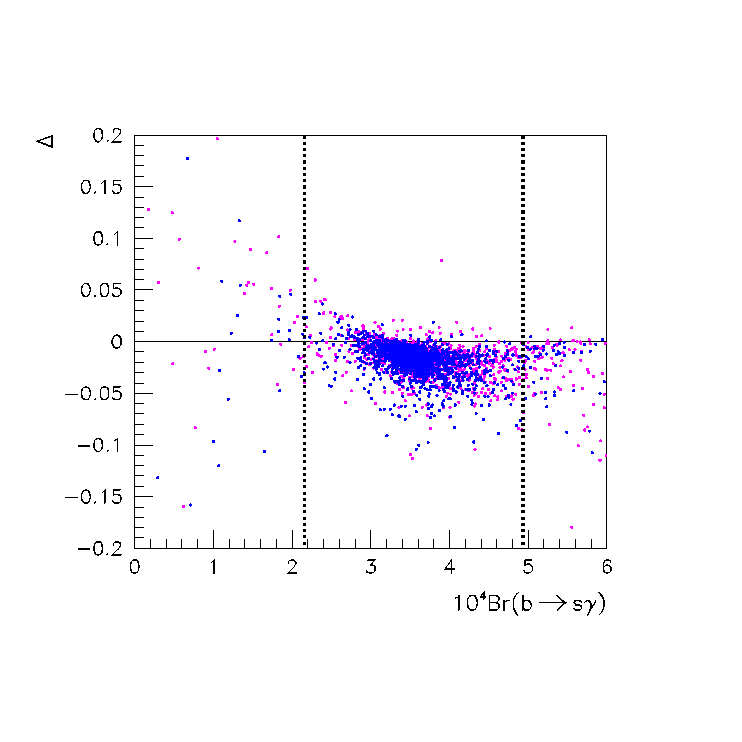
\includegraphics[width=8cm]{bsgiso.eps}
\vspace{-.3cm}
\caption{ Relative difference for $B(\bar{B}\rightarrow s\gamma)$ between micromegas$2.4$ and superIso$3.1$.
the vertical lines show the $3\sigma$ experimentally measured value.
}
\end{figure}


\begin{thebibliography}{}



%\cite{Belanger:2001fz}
\bibitem{Belanger:2001fz}
  G.~Belanger, F.~Boudjema, A.~Pukhov and A.~Semenov,
  %``micrOMEGAs: A program for calculating the relic density in the MSSM,''
  Comput.\ Phys.\ Commun.\  {\bf 149} (2002) 103
  [arXiv:hep-ph/0112278].
  %%CITATION = CPHCB,149,103;%%

%\cite{Belanger:2004yn}
\bibitem{Belanger:2004yn}
  G.~Belanger, F.~Boudjema, A.~Pukhov and A.~Semenov,
  %``micrOMEGAs: Version 1.3,''
  Comput.\ Phys.\ Commun.\  {\bf 174} (2006) 577
  [arXiv:hep-ph/0405253].
  %%CITATION = CPHCB,174,577;%%

%\cite{Belanger:2006is}
\bibitem{Belanger:2006is}
  G.~Belanger, F.~Boudjema, A.~Pukhov and A.~Semenov,
  %``micrOMEGAs2.0: A program to calculate the relic density of dark matter  in
  %a generic model,''
  Comput.\ Phys.\ Commun.\  {\bf 176} (2007) 367
  [arXiv:hep-ph/0607059].
  %%CITATION = CPHCB,176,367;%%

%\cite{Belanger:2008sj}
\bibitem{Belanger:2008sj}
  G.~Belanger, F.~Boudjema, A.~Pukhov and A.~Semenov,
  %``Dark matter direct detection rate in a generic model with micrOMEGAs2.2,''
  Comput.\ Phys.\ Commun.\  {\bf 180} (2009) 747
  [arXiv:0803.2360 [hep-ph]].
  %%CITATION = CPHCB,180,747;%%

\bibitem{Belanger:2010gh}
  G.~Belanger, F.~Boudjema, P.~Brun, A.~Pukhov, S.~Rosier-Lees, P.~Salati and A.~Semenov,
  %``Indirect search for dark matter with micrOMEGAs2.4,''
  arXiv:1004.1092 [hep-ph].
  %%CITATION = ARXIV:1004.1092;%%

%\cite{Allanach:2008qq}
\bibitem{Allanach:2008qq}
  B.~Allanach {\it et al.},
  %``SUSY Les Houches Accord 2,''
  Comput.\ Phys.\ Commun.\  {\bf 180} (2009) 8
  [arXiv:0801.0045 [hep-ph]].
  %%CITATION = CPHCB,180,8;%%

%\cite{Hugonie:2007vd}
\bibitem{Hugonie:2007vd}
  C.~Hugonie, G.~Belanger and A.~Pukhov,
  %``Dark Matter in the Constrained NMSSM,''
  JCAP {\bf 0711} (2007) 009
  [arXiv:0707.0628 [hep-ph]].
  %%CITATION = JCAPA,0711,009;%%






%\cite{Belanger:2006qa}
\bibitem{Belanger:2006qa}
  G.~Belanger, F.~Boudjema, S.~Kraml, A.~Pukhov and A.~Semenov,
  %``Relic density of neutralino dark matter in the MSSM with CP violation,''
  Phys.\ Rev.\  D {\bf 73} (2006) 115007
  [arXiv:hep-ph/0604150].
  %%CITATION = PHRVA,D73,115007;%%



%\cite{Belanger:2005kh}
\bibitem{Belanger:2005kh}
  G.~Belanger, F.~Boudjema, C.~Hugonie, A.~Pukhov and A.~Semenov,
  %``Relic density of dark matter in the NMSSM,''
  JCAP {\bf 0509} (2005) 001
  [arXiv:hep-ph/0505142].
  %%CITATION = JCAPA,0509,001;%%




%\cite{Skands:2003cj}
\bibitem{Skands:2003cj}
  P.~Skands {\it et al.},
  %``SUSY Les Houches accord: Interfacing SUSY spectrum calculators, decay
  %packages, and event generators,''
  JHEP {\bf 0407} (2004) 036
  [arXiv:hep-ph/0311123].
  %%CITATION = JHEPA,0407,036;%%




%\cite{Pukhov:2004ca}
\bibitem{Pukhov:2004ca}
  A.~Pukhov,
  %``CalcHEP 3.2: MSSM, structure functions, event generation, batchs, and
  %generation of matrix elements for other packages,''
  arXiv:hep-ph/0412191.
  %%CITATION = HEP-PH/0412191;%%

%\cite{Semenov:2008jy}
\bibitem{Semenov:2008jy}
  A.~Semenov,
  %``LanHEP - a package for the automatic generation of Feynman rules in field
  %theory. Version 3.0,''
  Comput.\ Phys.\ Commun.\  {\bf 180} (2009) 431
  [arXiv:0805.0555 [hep-ph]].
  %%CITATION = CPHCB,180,431;%%

%\cite{Belanger:2007dx}
\bibitem{Belanger:2007dx}
  G.~Belanger, A.~Pukhov and G.~Servant,
  %``Dirac Neutrino Dark Matter,''
  JCAP {\bf 0801} (2008) 009
  [arXiv:0706.0526 [hep-ph]].
  %%CITATION = JCAPA,0801,009;%%

\bibitem{Eidelman:2004wy}
  S.~Eidelman {\it et al.}  [Particle Data Group],
  %``Review of particle physics,''
  Phys.\ Lett.\  B {\bf 592} (2004) 1.
  %%CITATION = PHLTA,B592,1;%%



%\cite{Ellwanger:2006rn}
\bibitem{Ellwanger:2006rn}
  U.~Ellwanger and C.~Hugonie,
  %``NMSPEC: A Fortran code for the sparticle and Higgs masses in the NMSSM with
  %GUT scale boundary conditions,''
  Comput.\ Phys.\ Commun.\  {\bf 177} (2007) 399
  [arXiv:hep-ph/0612134].
  %%CITATION = CPHCB,177,399;%%
  
  \bibitem{Ellwanger:2005dv}
  U.~Ellwanger and C.~Hugonie,
  %``NMHDECAY 2.0: An Updated program for sparticle masses, Higgs masses,
  %couplings and decay widths in the NMSSM,''
  Comput.\ Phys.\ Commun.\  {\bf 175} (2006) 290
  [arXiv:hep-ph/0508022].
  %%CITATION = CPHCB,175,290;%%
  
  \bibitem{Domingo:2007dx}
  F.~Domingo and U.~Ellwanger,
  %``Updated Constraints from $B$ Physics on the MSSM and the NMSSM,''
  JHEP {\bf 0712} (2007) 090
  [arXiv:0710.3714 [hep-ph]].
  %%CITATION = JHEPA,0712,090;%%
  
  
  \bibitem{Lee:2003nta}
  J.~S.~Lee, A.~Pilaftsis, M.~S.~Carena, S.~Y.~Choi, M.~Drees, J.~R.~Ellis and C.~E.~M.~Wagner,
  %``CPsuperH: A computational tool for Higgs phenomenology in the minimal
  %supersymmetric standard model with explicit CP violation,''
  Comput.\ Phys.\ Commun.\  {\bf 156} (2004) 283
  [arXiv:hep-ph/0307377].
  %%CITATION = CPHCB,156,283;%%

\bibitem{Lee:2007gn}
  J.~S.~Lee, M.~Carena, J.~Ellis, A.~Pilaftsis and C.~E.~M.~Wagner,
  %``CPsuperH2.0: an Improved Computational Tool for Higgs Phenomenology in the
  %MSSM with Explicit CP Violation,''
  Comput.\ Phys.\ Commun.\  {\bf 180} (2009) 312
  [arXiv:0712.2360 [hep-ph]].
  %%CITATION = CPHCB,180,312;%%
  
  \bibitem{CPSUPERH}
  J.S.~Lee, A. Pilaftsis, M.~Carena, S.Y.~Choi, M.~Drees, J.~Ellis, C. Wagner,\\
  \verb|http://www.hep.man.ac.uk/u/jslee/CPsuperH.html|.
  
  \bibitem{nmssmtools}
  U.~Ellwanger, J.~Gunion, C.~Hugonie,\\
  \verb|http://www.th.u-psud.fr/NMHDECAY/nmssmtools.html|.


\bibitem{Numerical}
W.~H.~Press, S.~A.~Teukolsky,
W.~T.~Vetterling and  B.~P.~ Flannery,  
"Numerical Recipes: The Art of Scientific Computing'', Cambridge University
Press (2007).

%\cite{Mahmoudi:2010iz}
\bibitem{Mahmoudi:2010iz}
  F.~Mahmoudi {\it et al.},
  %`Flavour Les Houches Accord: Interfacing Flavour related Codes,''
  arXiv:1008.0762 [hep-ph].
  %%CITATION = ARXIV:1008.0762;%%

%\cite{Arbey:2011zz}
\bibitem{Arbey:2011zz}
  A.~Arbey and F.~Mahmoudi,
  %`SuperIso Relic v3.0: A program for calculating relic density and flavour
  %physics observables: Extension to NMSSM,''
  Comput.\ Phys.\ Commun.\  {\bf 182} (2011) 1582.
  %%CITATION = CPHCB,182,1582;%%

\bibitem{Misiak:2006zs}
  M.~Misiak, H.~M.~Asatrian, K.~Bieri, M.~Czakon, A.~Czarnecki, T.~Ewerth, A.~Ferroglia, P.~Gambino {\it et al.},
  %``Estimate of B(anti-B ---> X(s) gamma) at O(alpha(s)**2),''
  Phys.\ Rev.\ Lett.\  {\bf 98 } (2007)  022002.
  [hep-ph/0609232].

\bibitem{Misiak:2006ab}
  M.~Misiak, M.~Steinhauser,
  %``NNLO QCD corrections to the anti-B ---> X(s) gamma matrix elements using interpolation in m(c),''
  Nucl.\ Phys.\  {\bf B764 } (2007)  62-82.
  [hep-ph/0609241].

\bibitem{Gambino:2008fj}
  P.~Gambino, P.~Giordano,
  %``Normalizing inclusive rare B decays,''
  Phys.\ Lett.\  {\bf B669 } (2008)  69-73.
  [arXiv:0805.0271 [hep-ph]].

\bibitem{Yao:2006px}
  W.~M.~Yao {\it et al.} [ Particle Data Group Collaboration ],
  %``Review of Particle Physics,''
  J.\ Phys.\ G {\bf G33 } (2006)  1-1232.

\bibitem{Nakamura:2010zzi}
  K.~Nakamura {\it et al.} [ Particle Data Group Collaboration ],
  %``Review of particle physics,''
  J.\ Phys.\ G {\bf G37 } (2010)  075021.
  
  
\end{thebibliography}
\end{document}



\
